\documentclass[12pt, a4paper, oneside]{ctexart}
\usepackage{amsmath, amsthm, amssymb, bm, color, graphicx, geometry, mathrsfs,extarrows, braket, booktabs, array, xcolor, fontspec, appendix, float, subfigure, wrapfig, enumitem}
\usepackage[colorlinks,linkcolor=red,anchorcolor=blue,citecolor=blue,urlcolor=blue,menucolor=black]{hyperref}

%%%% 设置中文字体 %%%%
\setCJKmainfont{方正新书宋_GBK.ttf}[ BoldFont = 方正小标宋_GBK, ItalicFont = 方正楷体_GBK]
%%%% 设置英文字体 %%%%
\setmainfont{Times New Roman}
\setsansfont{Calibri}
\setmonofont{Consolas}

%%%% 设置代码块 %%%%
% 在vscode中使用minted需要先配置python解释器, Ctrl+Shift+P, 输入Python: Select Interpreter选择安装了Pygments的Python版本. 再在setting.json中xelatex和pdflatex的参数中加入 "--shell-escape", 即可
% TeXworks中配置方法参考: https://blog.csdn.net/RobertChenGuangzhi/article/details/108140093
\usepackage{minted}
\renewcommand{\theFancyVerbLine}{
    \sffamily\textcolor[rgb]{0.5,0.5,0.5}{\scriptsize\arabic{FancyVerbLine}}} % 修改代码前序号大小
% 加入不同语言的代码块
\newmintinline{cpp}{fontsize=\small, linenos, breaklines, frame=lines}
\newminted{cpp}{fontsize=\small, linenos, breaklines, frame=lines}
\newmintedfile{cpp}{fontsize=\small, linenos, breaklines, frame=lines}
\newmintinline{matlab}{fontsize=\small, linenos, breaklines, frame=lines}
\newminted{matlab}{fontsize=\small, mathescape, linenos, breaklines, frame=lines}
\newmintedfile{matlab}{fontsize=\small, linenos, breaklines, frame=lines}
\newmintinline{python}{fontsize=\small, linenos, breaklines, frame=lines, python3}  % 使用\pythoninline{代码}
\newminted{python}{fontsize=\small, escapeinside=||, mathescape=true, linenos, breaklines, python3}  % 使用\begin{pythoncode}代码\end{pythoncode}
\newmintedfile{python}{fontsize=\small, linenos, breaklines, frame=lines, python3}  % 使用\pythonfile{代码地址}
% 使用数学公式方法:|$公式$|

%%%% 设置行间距与页边距 %%%%
\linespread{1.2}
\geometry{left=2.5cm, right=2.5cm, top=2.5cm, bottom=2.5cm}

%%%% 定理类环境的定义 %%%%
\newtheorem{example}{例}            % 整体编号
\newtheorem{theorem}{定理}[section] % 定理按section编号
\newtheorem{definition}{定义}
\newtheorem{axiom}{公理}
\newtheorem{property}{性质}
\newtheorem{proposition}{命题}
\newtheorem{lemma}{引理}
\newtheorem{corollary}{推论}
\newtheorem{remark}{注解}
\newtheorem{condition}{条件}
\newtheorem{conclusion}{结论}
\newtheorem{assumption}{假设}
\numberwithin{equation}{section}  % 公式按section编号 (公式右端的小括号)
\newtheorem{algorithm}{算法}

\newsavebox{\nameinfo}
\newenvironment{myTitle}[1]{
    \begin{center}
    {\zihao{-2}\bf #1\\}
    \zihao{-4}\it
}{\end{center}}  % \begin{myTitle}{标题内容}作者信息\end{myTitle}
\newcounter{problem}  % 问题序号计数器
\newenvironment{problem}[1][]{\stepcounter{problem}\par\noindent\textbf{题目\arabic{problem}. #1}}{\smallskip\par}
\newenvironment{solution}[1][]{\par\noindent\textbf{#1解答. }}{\smallskip\par}  % 可带一个参数表示题号\begin{solution}{题号}
\newenvironment{note}{\par\noindent\textbf{注记. }}{\smallskip\par}

%%%% 图片相对路径 %%%%
\graphicspath{{figure/}} % 当前目录下的figure文件夹, {../figure/}则是父目录的figure文件夹
\setlength{\abovecaptionskip}{-0.2cm}  % 缩紧图片标题与图片之间的距离
\setlength{\belowcaptionskip}{0pt} 

%%%% 缩小item,enumerate,description两行间间距 %%%%
\setenumerate[1]{itemsep=0pt,partopsep=0pt,parsep=\parskip,topsep=5pt}
\setitemize[1]{itemsep=0pt,partopsep=0pt,parsep=\parskip,topsep=5pt}
\setdescription{itemsep=0pt,partopsep=0pt,parsep=\parskip,topsep=5pt}

\everymath{\displaystyle} % 默认全部行间公式, 想要变回行内公式使用\textstyle
\DeclareMathOperator*\uplim{\overline{lim}}     % 定义上极限 \uplim_{}
\DeclareMathOperator*\lowlim{\underline{lim}}   % 定义下极限 \lowlim_{}
\DeclareMathOperator*{\argmax}{arg\,max}  % 定义取最大值的参数 \argmax_{}
\DeclareMathOperator*{\argmin}{arg\,min}  % 定义取最小值的参数 \argmin_{}
\let\leq=\leqslant % 简写小于等于\leq (将全部leq变为leqslant)
\let\geq=\geqslant % 简写大于等于\geq (将全部geq变为geqslant)

%%%% 一些宏定义 %%%%
\def\bd{\boldsymbol}        % 加粗(向量) boldsymbol
\def\disp{\displaystyle}    % 使用行间公式 displaystyle(默认)
\def\tsty{\textstyle}       % 使用行内公式 textstyle
\def\sign{\text{sign}}      % sign function
\def\wtd{\widetilde}        % 宽波浪线 widetilde
\def\R{\mathbb{R}}          % Real number
\def\N{\mathbb{N}}          % Natural number
\def\Z{\mathbb{Z}}          % Integer number
\def\Q{\mathbb{Q}}          % Rational number
\def\C{\mathbb{C}}          % Complex number
\def\K{\mathbb{K}}          % Number Field
\def\P{\mathbb{P}}          % Polynomial
\def\N{\mathbb{N}}          % Natural number
\def\Z{\mathbb{Z}}          % Integer number
\def\E{\mathbb{E}}          % Exception
\def\var{\text{Var}}        % Variance
\def\bias{\text{bias}}      % bias
\def\d{\mathrm{d}}          % differential operator
\def\e{\mathrm{e}}          % Euler's number
\def\i{\mathrm{i}}          % imaginary number
\def\re{\mathrm{Re}}        % Real part
\def\im{\mathrm{Im}}        % Imaginary part
\def\res{\mathrm{Res}}      % Residue
\def\L{\mathcal{L}}         % Loss function
\def\O{\mathcal{O}}         % 时间复杂度
\def\wdh{\widehat}          % 宽帽子 widehat
\def\ol{\overline}          % 上横线 overline
\def\ul{\underline}         % 下横线 underline
\def\add{\vspace{1ex}}      % 增加行间距
\def\del{\vspace{-1.5ex}}   % 减少行间距

%%%% 正文开始 %%%%
\begin{document}

%%%% 以下部分是正文 %%%%  
\clearpage
\begin{myTitle}{数学建模期末报告-背包问题}
    吴天阳\ 2204210460\ 强基数学002
\end{myTitle}

\section{背包问题}
背包问题(Knapsack problem)是一种组合优化的NP完全问题. 问题基本表述为:给定一组物品,每种物品具有自己的体积与价值,在有限的体积内,如何选择,使得物品的总价值达到最大.

该问题在实际中具有非常广泛的应用,例如如何打包行李使得最大化行李价值且不超载、资源分配问题:从多个项目中具有时间或预算的限制,在相同时间或预算内达到最大的价值. 所以研究背包问题十分有价值,这里以经典的《背包九讲》对基础的三种背包算法进行学习.

注:下文中小数默认\textbf{向下取整}.
\subsection{01背包问题}
\paragraph*{问题}总共有$N$件物品和一个容量大小为$V$的背包,其中第$i$件物品的容量为$c[i]$,价值为$w[i]$. 求解在不超过背包容量的前提下最大化物品价值.
\paragraph*{分析}该问题是最基础的背包问题,由于每个物品只能选择装与不装,即对应0与1的状态,所以也称为01背包问题.

定义状态数组:$dp[i][j]$表示前$i$件物品放入容量为$j$的背包可获得的最大价值. 则其状态转移方程为
\begin{equation*}
        dp[i][j] = \max\left\{dp[i-1][j],dp[i-1][j-c[i]]+w[i]\right\}
\end{equation*}
动态规划本质是考虑当前状态与之前状态的关系,通过之前已有的状态通过转移方程得到当前状态的值. 我们考虑当前第$i$个物品是否放入背包:如果不放,则问题转化为前$i-1$个物品放入大小为$j$的背包可获得的最大价值;如果放,则问题转化为前$i-1$个物品放入大小为$j-c[i]$大小的背包可获得的最大价值加上当前物品的价值$w[i]$. 于是,再对这两项取$\max$即可得到上述状态转移方程.

\paragraph*{优化}上述算法的时间复杂度与空间复杂度均为$\O(VN)$,但是空间复杂度可以优化到$\O(N)$. 首先分析上述算法的具体实现方法
\begin{pythoncode}
for i=1 to N do
    for j=c[i] to V do
        dp[i][j] = max(dp[i-1][j], dp[i-1][j-c[i]]+w[i])
\end{pythoncode}
如果我们考虑反向推导第二维循环,那么我们就可以通过一维数组完成上述操作
\begin{pythoncode}
for i=1 to N do
    for j=V to c[i] do
        dp[j] = max(dp[j], dp[j-c[i]]+w[i])
\end{pythoncode}
因为如果反向枚举,我们仍可以保证$dp[j-c[i]]$就是原来的$dp[i-1][j-c[i]]$,即前$i-1$个物品的对应的状态.

由于01背包用途广泛,所以我们引入如下函数专门用于处理一件01背包中的物品
\begin{pythoncode}
def ZeroOnePack(cost, weight)  # cost为物品大小, weight为物品的价值
    for v=V to cost do
        dp[v] = max(dp[v], dp[v-cost]+weight)
\end{pythoncode}
有了这个过程后,01背包可以简写成如下形式
\begin{pythoncode}
for i=1 to N do
    ZeroOnePack(c[i], w[i])
\end{pythoncode}
\subsection{完全背包问题}
\paragraph*{问题}总共有$N$件物品和一个容量大小为$V$的背包,每种物品都可以无限次使用. 其中第$i$件物品的容量为$c[i]$,价值为$w[i]$. 求解在不超过背包容量的前提下最大化物品价值.
\paragraph*{分析}该问题与01背包问题非常类似. 根据01背包的状态转移方程,我们可以类似定义状态数组:$dp[i][j]$表示前$i$件物品放入容量为$j$的背包可获得的最大价值,则其状态转移方程为
\begin{equation}\label{eq-1}
    dp[i][j] = \max\{dp[i-1][j], dp[i-1][j-k\cdot c[i]]+k\cdot w[i]: k\cdot c[i]\leq j\}
\end{equation}
当前状态$dp[i][j]$可以通过选择$k$个第$i$种物品,于是可以从$dp[i-1][j-k\cdot c[i]]$处进行转移. 这根据01背包的问题相同,类似求解思路可以得到时间复杂度为$\O(V\sum_{i=1}^N\frac{V}{c[i]})$.
\paragraph*{优化}由于每件物品数量具有无穷多个,所以如果我们考虑第$i$件物品不从第$i-1$个物品的状态进行转移,而是直接通过当前物品的上一个状态进行转移,即以下转移方程
\begin{equation}\label{eq-2}
    dp[i][j] = \max\{dp[i-1][j], dp[i][j-c[i]]+w[i]\}
\end{equation}
首先,理性分析下上述转移方程的含义,由于每个物品能够选择无限多次. 所以,当前第$dp[i][j]$个物品的状态可以直接通过当前物品的$j-c[i]$的容量大小进行转移,这就相当于可以重复选择当前物品多次.

下面我们来证明该转移方程的结果与(\ref{eq-1})的结果相同,假设(\ref{eq-1})式中取到$k$时有最大值,也即是
\begin{align*}
    &\ dp[i-1][j-k\cdot c[i]] > dp[i-1][j-(k+1)\cdot c[i]]+w[i] > dp[i][j-(k+1)j\cdot c[i]]\\
    \Rightarrow&\ dp[i][j-k\cdot c[i]] = dp[i-1][j-k\cdot c[i]]
\end{align*}
所以存在一种转移链使得
\begin{align*}
    dp[i][j] =&\ dp[i][j-c[i]] + w[i] = dp[i][j-2c[i]]+2w[i] =\cdots\\
    =&\  dp[i][j-k\cdot c[i]]+k\cdot w[i] = dp[i-1][j-k\cdot c[i]] + k\cdot w[i]
\end{align*}
于是转移方程(\ref{eq-1})与(\ref{eq-2})完全等价,且复杂度为$\O(VN)$,和01背包相同. 代码实现如下
\begin{pythoncode}
for i=1 to N do
    for j=c[i] to V do
        dp[i][j] = max(dp[i-1][j], dp[i][j-c[i]]+w[i])
\end{pythoncode}
类似地可以编写专门处理一件完全背包中的物品
\begin{pythoncode}
def CompletePack(i, cost=c[i], weight=w[i])  # 当前处理第i件物品
    for j=1 to V do
        dp[i][v] = max(dp[i-1][v], dp[i][v-c[i]]+w[i])
\end{pythoncode}
对于与01背包的区别,我们可以观察到仅有第二层循环的遍历顺序不同,转移方程上有微小变化.

\paragraph*{其他优化技巧}
一个直观的优化方法,假设物品$i$的容量大且价值低与另一个物品$j$,也即$c[i]\geq c[j]$且$w[i] \leq w[j]$,则物品$i$一定不会被选中. 因为假如能够选中物品$i$,则一定可以通过选物品$j$代替物品$i$使得总价值达到更大.

第二种优化方法,虽然不如第一种优化方法,但仍具有思考价值. 如果我们将一种物品$i$,打包的思路合成一个物品,则一共能打包为$\lfloor V/c[i] \rfloor$个物品,设$k=1,2,\cdots, \lfloor V/c[i] \rfloor$,则第$k$个物品的容量为$k\cdot c[i]$,价值为$k\cdot w[i]$,则打包后的物品总数目为$\sum_{i=1}^N\frac{V}{c[i]}$. 于是可以将问题转化为求解01背包,但是这样的时间复杂度并没有优化,仍和转移方程(\ref{eq-1})的时间复

进一步思考,如果一件物品的打包不是一个一个的打包,而是以2进制进行打包,也即$k=1,2,\cdots, \lfloor\log V/c[i]\rfloor$,第$k$个的容量为$2^k\cdot c[i]$,价值为$2^k\cdot w[i]$,这样就打包出$\sum_{i=1}^N\log \frac{V}{c[i]}$个物品,因为可以通过是否选择一个二进制数来得到所有数字,所以和第一种方式结果相同. 再使用01背包方式求解,总复杂度为$\O(V\cdot \sum_{i=1}^N\log \frac{V}{c[i]})$.

\subsection{多重背包问题}
\paragraph*{问题}总共有$N$件物品和一个容量大小为$V$的背包. 第$i$种物品最多有$a[i]$件可以选取,第$i$种物品的容量均为$c[i]$,价值为$w[i]$. 求解在不超过背包容量的前提下最大化物品价值.
\paragraph*{分析}该问题与完全背包问题非常类似. 根据完全背包的思路$k$会被两个上界所限制住
\begin{equation}\label{eq-3}
    dp[i][j] = \max\left\{dp[i-1][j], dp[i-1][j-k\cdot c[i]]+k\cdot w[i]: k\leq \min\left\{a[i],\frac{V}{c[i]}\right\}\right\}
\end{equation}
总时间复杂度为$\O(V\cdot \sum_{i=1}^Na[i])$.

\paragraph*{优化}我们可以通过类似完全背包第二种优化方法,将物品进行二进制合并,然后通过二进制数合并得到$1,\cdots, a[i]$每个数的组合. 假设打包为$k+1$组,则前$k-1$个包大小分别为$1,2^1,2^2,\cdots, 2^{k-1}$,则总计为$\sum_{i=0}^{k-1}2^i = 2^k-1$,于是最后一个包大小是$a[i] - 2^k+1$,且满足$k$是使得$a[i]-2^k+1 > 0$的最大值,即$2^k\leq a[i]\Rightarrow k = \log a[i]$. 进而转化为01背包问题,从而总时间复杂度变为$\O(V\cdot \sum_{i=1}^N\log a[i])$. 多重背包问题中处理一个物品的代码如下:
\begin{pythoncode}
def MultiplePack(i, cost=c[i], weight=w[i], amount=a[i])  # 当前处理第i件物品
    if cost * amount >= V do
        CompletePack(i, cost, weight)  # 当c[i]*a[i]大于当前包容量, 则等价于完全背包问题
    k = 1  # 当前打包的大小
    while k < amount do
        ZeroOnePack(k * cost, k * weight)
        amount = amount - k
        k = k * 2
    ZeroOnePack(amount * cost, amount * weight)
\end{pythoncode}
\paragraph*{单调队列优化}利用单调队列优化,可以将时间复杂度降低到$\O(VN)$. 此算法是基于动态规划(\ref{eq-3})式的优化算法,我们观察对于容量为$j$,则当前容量只会和$j-c[i],j-2c[i],\cdots, j-a[i]\cdot c[i]$相关,也就是$\bar{j}$在模$c[i]$下的等价类,取最近的$a[i]$项. 所以利用这一性质,我们可以将整个背包容量用模$c[i]$的等价类进行划分,在每个等价类中分别计算转移方程的最大值.

考虑如何在$\O(1)$的复杂度下获得当前等价类中的最大dp值. 在一个等价类中,我们从左至右滑动一个大小为$a[i]$的滑动窗口,并用单增的单调队列维护当前滑动窗口的最大值,加入当前滑动窗口最右侧端点值为$j$,则$dp[j]$为当前单调队列队首对应的dp值加上当前物品的价值.

单调队列具体实现方法:考虑用单调队列维护一个对应状态值单调递增的\textbf{下标}队列,保证队首元素处于当前滑动窗口内,当前元素加入队列时,保证队尾的状态值大于当前加入的状态值. 具体实现请见代码:
\begin{pythoncode}
def MultiplePackQueue(i, cost=c[i], weight=w[i], amount=a[i])  # 当前处理第i件物品
    initialize queue  # 创建一个空的队列
    for j=0 to cost do  # 枚举当前等价类的开头
        for k=j to V by cost do  # 枚举等价类中的元素k
            value = dp[i-1][k] - (k-j) / cost * weight  # 定义当前所需维护的权重
            while (queue not empty) and (queue.front.position < k - amount * cost) do  # 若首元素已经超出了当前滑动窗口大小, 弹出
                pop queue.front
            while (queue not empty) and (queue.back.value < value) do  # 若队尾元素的权重小于当前权重,弹出
                pop queue.back
            if queue not empty do
                dp[i][k] = max(dp[i-1][k], dp[i-1][queue.head.position] + (k-queue.head.position) / cost * weight)
            else do
                dp[i][k] = dp[i-1][k]
            push (position=k, value=value) into queue  # 将当前新节点加入单调队列
\end{pythoncode}
上述过程虽然是三层for循环,但是第二、三层for循环是对$1,\cdots,N$的一个划分,所以总复杂度仍为$\O(VN)$.
\section*{总结}
通过这三种背包的学习,基本掌握了解决背包问题的基本思想,主要为通过设计动态规划数组与状态转移方程,通过数学建模的方法将原问题转化为数学中离散的最优化问题. 在01背包的基础上,通过可以多次选取物品,衍生出完全背包(可无限次选取)与多重背包(每种物品数目有限)两种背包问题,一种有效的通用方法为二进制打包,即将多个物品打包以2的幂次打包成为一个物品,再利用01背包算法求解. 而他们都分别具有更为高效的算法,完全背包通过调整转移方程进行优化,多重背包则是通过划分为子问题、通过滑动窗口结合单调队列维护最大值进行求解.

通过这三种问题的研究,对数学建模有了更深刻的认识,通过将实际问题转化为数学最优化问题,再从一个问题推广到求解其他类似问题,更进一步考虑不同优化方法对算法进行改进. 这提示我们要不断思考与改进现有的模型,并学会在已有的基础上进行创新,从而得到更高效的算法.
\end{document}

\iffalse
%%%% 表格模板 %%%%
\renewcommand\arraystretch{0.8} % 设置表格高度为原来的0.8倍
\begin{table}[!htbp] % table标准
    \centering % 表格居中
    \begin{tabular}{p{1cm}<{\centering}p{1cm}<{\centering}p{3cm}<{\centering}p{5cm}<{\centering}} % 设置表格宽度
    %\begin{tabular}{cccc}
        \toprule
        $x_i$ & $f[x_1]$ & $f[x_i, x_{i+1}]$ & $f[x_i, x_{i+1}, x_{i+2}]$ \\
        \midrule
        $x_0$ & $f(x_0)$ &                  &                          \\
        $x_0$ & $f(x_0)$ & $f'(x_0)$        &                          \\
        $x_0$ & $f(x_1)$ & $\frac{f(x_1)-f(x_0)}{x_1-x_0}$ & $\frac{f(x_1)-f(x_0)}{(x_1-x_0)^2}-\frac{f'(x_0)}{x_1-x_0}$\\
        \bottomrule
    \end{tabular}
\end{table}

%%%% 文字环绕图片, 标题加注释 %%%%
{ % 一般将文字环绕部分的图和文字, 用大括号括起来, 避免对文字外的格式发生影响
\begin{wrapfigure}[13]{r}{.5\linewidth} % 文字环绕行数为13行, 图片靠右 (l为靠左), 图片占0.5的行宽
    \centerin右
    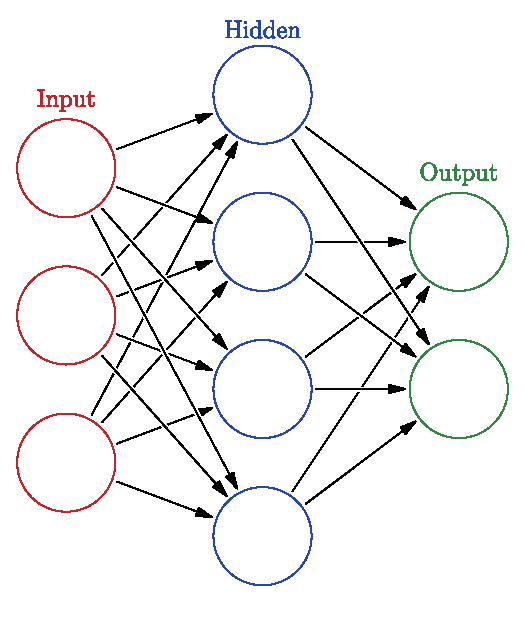
\includegraphics[scale=0.7]{neural_network.eps} % scale=0.7按比例缩放70%
    \caption{神经网络结构\protect\footnotemark[1]} % 记得加\protect, 设置1号脚标
    \label{figure-神经网络结构}
\end{wrapfigure}
\footnotetext[1]{图片来源: \url{https://en.wikipedia.org/wiki/File:Colored_neural_network.svg}}
文字文字
}

%%%% 普通图片, 标题加注释 %%%%
\begin{figure}[htbp] % h: 当前位置, t: 顶部, b: 底部, p: 浮动页, 这样组合指的是使用这个顺序进行排版
    \centering
    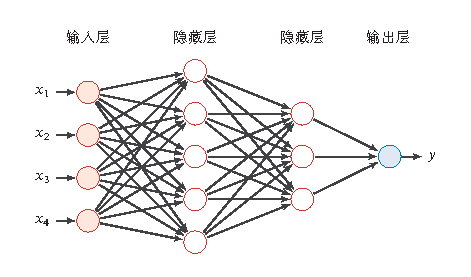
\includegraphics[scale=0.5]{前馈神经网络.eps}
    \caption{前馈神经网络\protect\footnotemark[1]}
    \label{figue-前馈神经网络}
\end{figure}
\footnotetext[1]{图片来源: 邱锡鹏, 神经网络与深度学习 \cite{ref-qxp}, 第92页}

%%%% 多组图 %%%%
    \begin{figure}[htbp]
        \centering
        \subfigure[迭代1次]  % 子图的标题
        {
            % 如果一行放三个图改成0.3\linewidth即可
            \begin{minipage}[b]{.45\linewidth}  % 0.45排版行距, 即一行放2个图, 一行放不下就换行
                \centering
                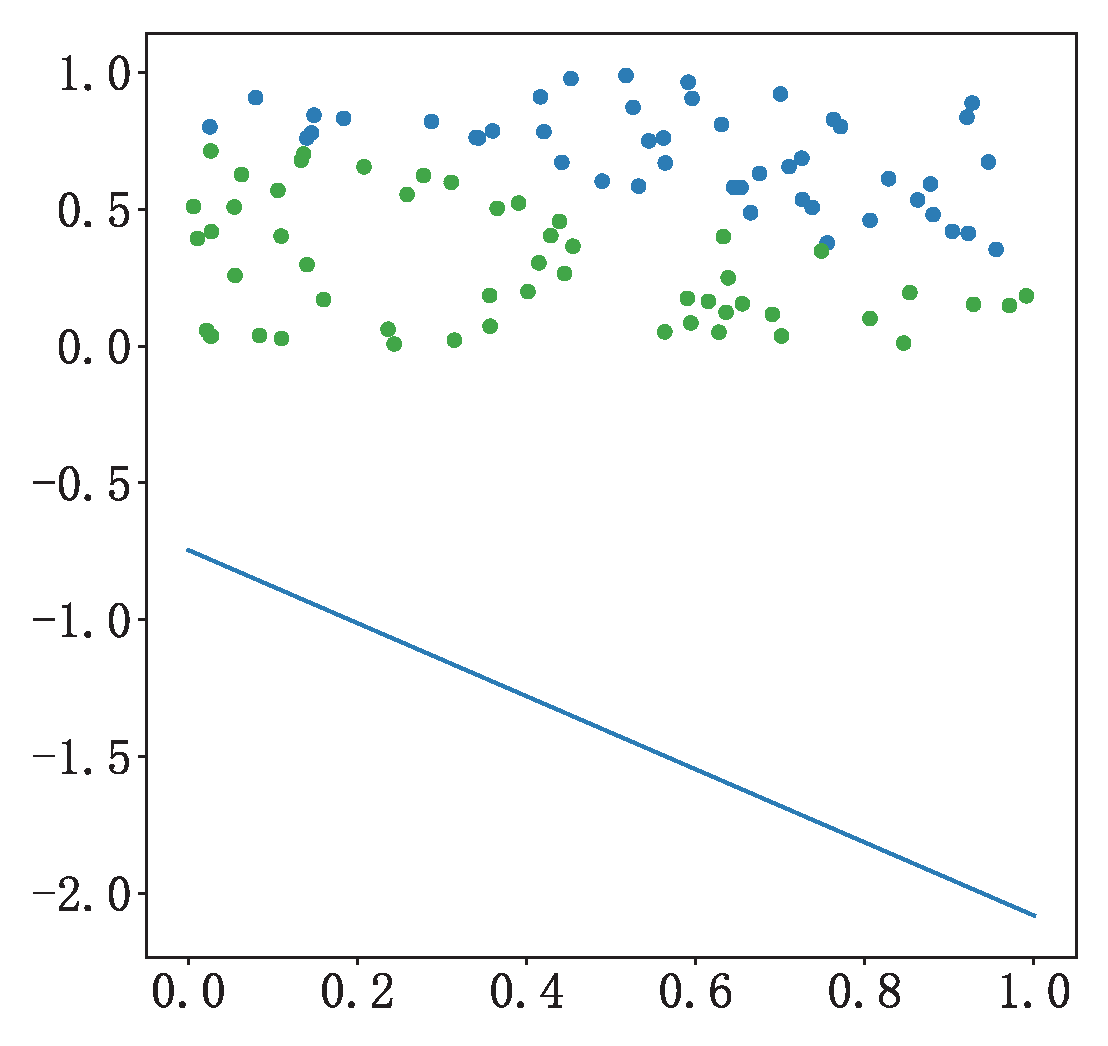
\includegraphics[scale=0.35]{1.eps}
            \end{minipage}
        }
        \subfigure[迭代100次]
        {
            \begin{minipage}[b]{.45\linewidth}
                \centering
                \includegraphics[scale=0.35]{100.eps}
            \end{minipage}
        }
        \subfigure[迭代500次]
        {
            \begin{minipage}[b]{.45\linewidth}
                \centering
                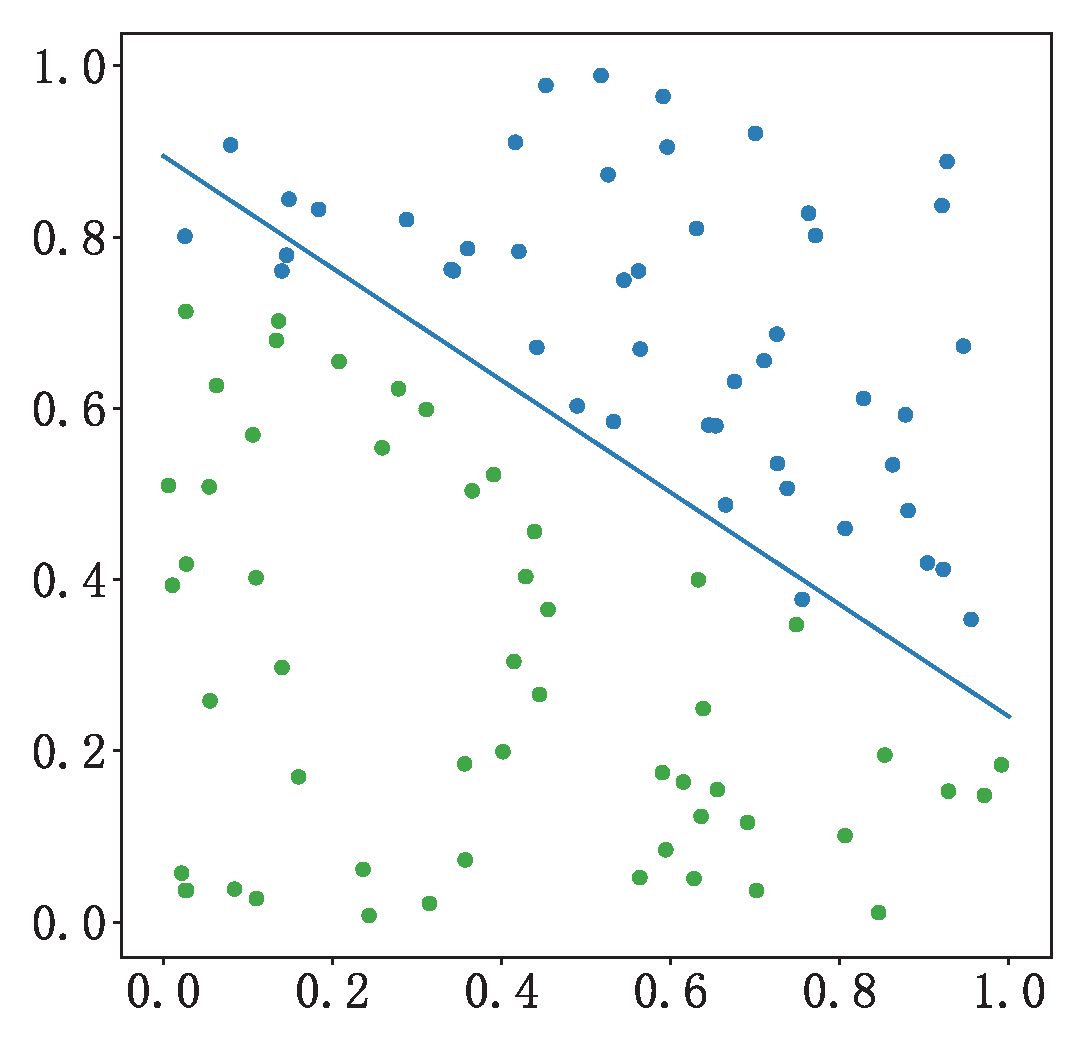
\includegraphics[scale=0.35]{500.eps}
            \end{minipage}
        }
        \subfigure[迭代2000次]
        {
            \begin{minipage}[b]{.45\linewidth}
                \centering
                \includegraphics[scale=0.35]{2000.eps}
            \end{minipage}
        }
        \caption{迭代过程图}
        \label{figure-迭代过程图}
    \end{figure}
\fi
